\documentclass[logo,reportComp]{thesis}
\usepackage[cpp,linenum]{mypackage}

\title{编译原理实验二}
\subtitle{Flex提取C/C++程序整数和浮点数}
\school{数据科学与计算机学院}
\author{陈鸿峥}
\classname{17大数据与人工智能}
\stunum{17341015}
\headercontext{编译原理实验作业}

\begin{document}

\maketitle
% https://www.geeksforgeeks.org/check-given-string-valid-number-integer-floating-point-java-set-2-regular-expression-approach/
% https://blog.ostermiller.org/finding-comments-in-source-code-using-regular-expressions/
% https://stackoverflow.com/questions/19488772/non-greedy-regular-expression-matching-in-flex

\section{实验目的}
用Flex实现下面的功能:
输入一个合法的C/C++程序,提取出程序中的整数和浮点数,并统计各自出现的次数。
注意像变量名或函数名中包含的数字不应统计进去。

加分项:忽略掉注释里面的整数和浮点数。

提交一份简要的实验报告,实验报告应包括程序功能描述、Flex文件的代码和若干实验的结果截图。

\section{程序功能描述}
由老师上周提供的Flex模板,只需修改前面初始化变量和正则表达式匹配的部分即可。
后面主函数部分采用文件读入,并将结果输出。

由于要统计整数和浮点数的数量,因此在初始化区初始两个计数变量\texttt{cnt\_int}和\texttt{cnt\_float},并赋初值为$0$。

虽然只需要提取程序中的整数和浮点数,但是为了排除一些不被提取的情况,因此另外附加对变量名和注释的识别。

\subsection{识别整数}
对于整数,我们有下面的正则定义
\[\begin{aligned}
sign &\to + \mid - \mid \epsilon\\
digit &\to 0 \mid 1 \mid \cdots \mid 9\\
num &\to sign\;digit\;digit^*
\end{aligned}\]
因此可以得到正则表达式
\begin{center}
\verb'[+-]?[0-9][0-9]*'
\end{center}
其中\verb'?'代表零个或一个。

\subsection{识别浮点数}
对于浮点数,我们有如下定义
\[\begin{aligned}
sign &\to + \mid - \mid \epsilon\\
digit &\to 0 \mid 1 \mid \cdots \mid 9\\
digits &\to digit\; digit^*\\
optional\_fraction &\to .\; digits \mid \epsilon\\
optional\_exponent &\to ((E \mid e)\; (+ \mid - \mid epsilon)\; digits) \mid epsilon\\
num &\to sign\; digits\; optional\_fraction\; optional\_exponent
\end{aligned}\]

可得正则表达式为
\begin{center}
\verb'[+-]?[0-9]+(\.[0-9]+)?([Ee][+-]?[0-9]+)?'
\end{center}

注意浮点数表达式和整数表达式在Flex中放置的先后次序。
由于浮点数中必然包含整数,如果将浮点数的正则表达式放在前面,Flex则会提示整数的正则表达不会被匹配(warning, rule cannot be matched),因此应该先处理整数后处理浮点。
% https://www.cs.virginia.edu/~cr4bd/flex-manual/Diagnostics.html

\subsection{变量名处理}
由于C/C++的变量和函数名都是可以含有数字的,因此为了避免将这些变量名中的数字提取出来,需要在提取整数和浮点数之前先将这些变量名进行解析。

C/C++的变量名非常简单,大小写字母、数字加下划线,首个字符不能为数字,因此可得正则表达式
\begin{center}
\verb'[a-zA-Z_][a-zA-Z0-9]*'
\end{center}

\subsection{注释处理}
同样,对于注释中的数字我们也是不需要将其进行统计的,因此我们在\textbf{最开始}就应该对注释语句进行处理。
C/C++中有两种注释的写法,一种是行末的注释\verb'//',另一种是可跨行的注释\verb'/* */'。

对于前者,正则表达式非常简单
\begin{center}
\verb'(//.*)'
\end{center}

对于后者,则需要考虑到跨行的情况。
初步尝试可以得到下面的正则表达式,两侧是斜杠加星号,中间可以是任意字符,也包括了换行符
\begin{center}
\verb'/\*(.|[\r\n])*?\*/'
\end{center}
其中\verb'?'代表非贪心(non-greedy)匹配,意味着只要顺序第一个匹配上该子表达式,这个正则表达式就算匹配完成了,这样可以有效避免多个注释全部整合到一起的情况。
虽然这种Lazy模式的匹配在C++\verb'<regex>'库及大量文本编辑器中都支持,但是非常遗憾的是Flex并不提供这种特性,因此需要重新再对其修改。

不采用非贪心匹配的做法则和理论作业二的第二题比较类似,我们需要考虑中间出现多个星号的情况。
对于注释中间的字符
\begin{itemize}
	\item 要么不是星号,即\verb'[^*]'
	\item 要么是换行符,即\verb'[\r\n]'
	\item 要么星号后面不跟斜杠,而且这里的星号可以是一个或多个,有\verb'(\*+([^*/]|[\r\n]))'
\end{itemize}

整合起来得到
\begin{center}
\verb'/\*([^*]|[\r\n]|(\*+([^*/]|[\r\n])))*\*/'
\end{center}
这个正则表达式可以有效处理多行注释的情况。

再与前面的行末注释的表达式做或操作,即可得到最终匹配所有注释的正则表达式。

\subsection{完整代码}
将上述内容整合到一起,可得下面完整的\verb'lex.l'程序。
注意实现过程中需要将斜杠和星号进行转义输出。
\lstinputlisting{lex.l}

\section{实验结果}
我将\textbf{所有的测试样例}都整合进\verb'lex_test.cpp'文件中,如下所示。
\lstinputlisting{lex_test.cpp}

这里涵盖了以下这些测试样例:
\begin{itemize}
	\item 多行注释、多星号
	\item 注释内含数字、变量等
	\item 不同位置的多种不同注释(行内及行末)
	\item 科学计数法表示浮点数
	\item 类型名、变量名、结构体成员名含数字
	\item 数字前后空格数目不等
	\item 单一表达式内含多个数字
	\item 数字含符号
	\item 数字作为右值
	\item 数字以不同符号作为前导
\end{itemize}

运行结果如图\ref{fig:results}所示,可以看到我的分析器成功将程序中的整数和浮点数提取了出来,同时也排除了注释中的数字。
\begin{figure}[H]
\centering
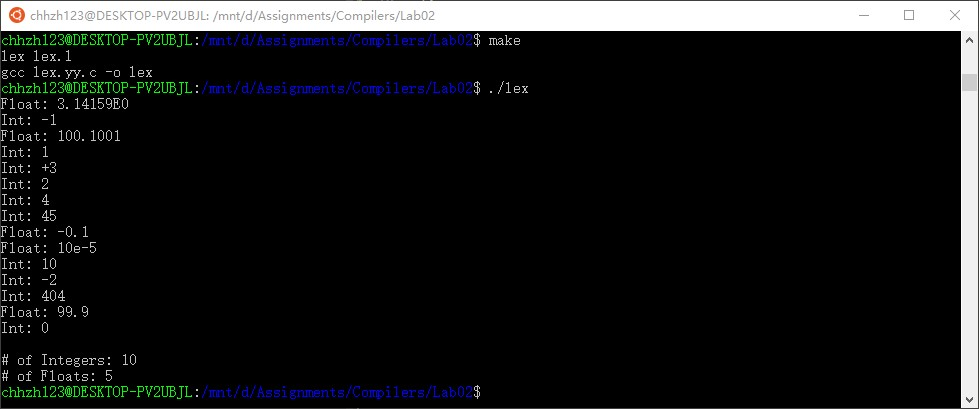
\includegraphics[width=\linewidth]{fig/results.jpg}
\caption{编译运行结果}
\label{fig:results}
\end{figure}

\end{document}